\section{Sorting}
\label{sec:sorting}

One of the most fundamental operations in computer science is sorting a sequence of elements. And as old as the problem is as numerous are the algorithms to solve it. These sorting algorithms differ in various aspects such as best, average and worst runtime or memory complexity, stability, the number of comparisons and swaps and whether the algorithm is a comparison sort or not.

The sort implementations provided by todays standard libraries are highly tuned achieving an optimal asymptotic runtime complexity which is $\mathcal{O}(n log n)$ for comparison based sorts. Examples would be variations of quick sort (C), merge sort (C++), intro sort (C++, .NET) or Timsort (Java, Python). All these algorithms are comparison sorts, thus requiring a method of comparing two elements of the input sequence. This comparison is often provided either by the language or standard library (e.g. $<$ operator) or by the programmer via a custom comparison function giving the flexibility to compare and sort any kind of elements.

Another class of sorting methods are integer sorting algorithms. These algorithms do not use comparisons to determine the order of elements but rely on more flexible integer arithmetic applied to the keys which should be sorted. Therefore, they can achieve a better asymptotic runtime complexity than comparison based ones. Popular algorithms of this kind are radix sort, counting sort and bucket sort. All of them running with $\mathcal{O}(n + k)$ or $\mathcal{O}(n * k)$ (where k is a constant) in linear time.
However, despite their key limitation, integer sorting algorithms also work on other kind of types as long as they can be represented as integers in binary (e.g. strings can be seen as byte array forming a (larger) integer).

Considering parallelizability and an eventual GPU implementation, sorting lies between matrix multiplication and prefix sum offering some degree of parallelism depending on the chosen algorithm. The following chapter will focus on the implementation of two widely chosen algorithms for GPU sorting. These are the comparison based bitonic sorting network and the integer sorting algorithm radix sort. To reduce code complexity (especially of the latter), the input array consists of unsigned 32 bit integers.


\subsection{CPU Implementations}

\subsubsection{C/C++ standard library routines}

As the later GPU implementations should be compared with well implemented and wide-spread CPU ones, the first step is to measure the performance of the standard library's routines.
Listing \ref{lst:sort_cpu_qsort} shows a typical usage of the \lstinline|qsort()| function provided by the stdlib header from C.

\lstset{basicstyle=\ttfamily{}\scriptsize{}}
\lstinputlisting[language=C++, caption=Sorting an array of unsigned integers using \lstinline!qsort()! from the C stdlib header., label=lst:sort_cpu_qsort, firstline=36, lastline=46]{code/sort/main.cpp}
\lstset{basicstyle=\ttfamily{}}

As qsort() is usually precompiled and part of the runtime library, a compare function has to be provided which is called for every comparison. This will probably slow down the run time when compared with the C++ \lstinline!std::sort()! which can use an existing overload of the $<$ operator or inline a provided compare function thanks to templates.
Listing \ref{lst:sort_cpu_sort} shows a typical call to the \lstinline!std::sort()! function template from the C++ algorithm header.

\lstset{basicstyle=\ttfamily{}\scriptsize{}}
\lstinputlisting[language=C++, caption=Sorting an array of unsigned integers using \lstinline!std::sort()! from the C++ algorithm header., label=lst:sort_cpu_sort, firstline=48, lastline=51]{code/sort/main.cpp}
\lstset{basicstyle=\ttfamily{}}

As the $<$ operator is defined for unsigned integer types no custom compare function has to be provided and no additional overhead is created for comparing elements.
The difference can be clearly seen in the benchmark chart in figure \ref{fig:sort_chart}. It takes \lstinline!qsort()! 14.746 seconds to sort a sequence of $2^{26}$ elements while \lstinline!std::sort()! only requires 9.039 seconds.

\subsubsection{Radix sort}

In contrast to the comparison based \lstinline!qsort()! and \lstinline!std::sort()! radix sort operates on the binary representation of the input elements in several passes. Originally, in each pass a bit of each input element is selected (starting with the least significant bit). The input elements are then split into two sequences (called buckets) according to the selected bit. This is done by creating a histogram holding the number of elements having the same bit value for each bit combination (0 or 1). After the histogram has been created it is exclusively scanned. The scanned histogram now holds the start index for each bucket. The input elements are permuted and moved into their corresponding buckets according to the selected bit. Elements with an equal bit are written into the same bucket in the same order as they appeared in the pass' input (each pass is stable). An auxiliary array is usually needed for this permute step. This procedure is repeated for every bit of the input elements. 

By only selecting one bit in each pass 32 passes are required to sort the input sequence (elements are 32 bit unsigned integers). In each pass the input array is iterated over two times and the histogram has to be scanned once. This accumulates to 64 iterations over the input sequence and 32 scans of a two element histogram making radix sort a linear algorithm but with a quite significant constant factor. This factor can be reduced by selecting several bits of each input element at once in each pass. As a result the number of passes decrease linearly with the number of selected bits (which is called radix and gives the algorithm its name). As a trade-off the size of the histogram increases by a power of two.

The CPU radix sort implementation used in the benchmarks is provided in listing \ref{lst:sort_cpu_radix}.

\lstset{basicstyle=\ttfamily{}\scriptsize{}}
\lstinputlisting[language=C++, caption=Sorting an array of unsigned integers using radix sort. The algorithm uses eight passes analyzing four bits each. The implementation is based on the radix sort sample shipped with AMD APP SDK \cite{amd_app_sdk}., label=lst:sort_cpu_radix, firstline=53, lastline=105]{code/sort/main.cpp}
\lstset{basicstyle=\ttfamily{}}

The implementation uses a relatively high radix of 16 which allows radix sort to finish in two passes. As a consequence, the histogram consists of $2^{16}$ elements occupying 256 KiB of memory but has to be scanned only two times.

The performance difference of radix sort to the previously presented comparison based algorithm is significant as seen in figure \ref{fig:sort_chart}. Although the high radix of 16 causes a large overhead on small input sizes (as the full $2^{16}$ element histogram has to be scanned independently of the input size), radix sort shows its strength on larger inputs. It catches up to \lstinline!std::sort()! at approximately 10,000 elements and then outdistances the library routine largely sorting $2^{26}$ elements in 0.884 seconds (compared to 9.039 seconds of \lstinline!std::sort()!).

\begin{figure}
\centering
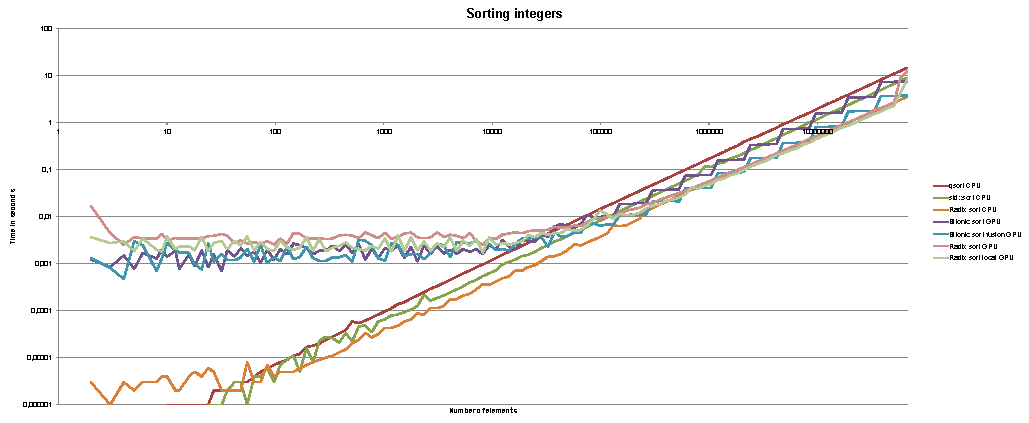
\includegraphics[width=\linewidth]{sort_chart}
\caption{Benchmark of several sort implementations. The chart is based on the benchmark data in appendix chapter \ref{sec:sort_chart_data}.}
\label{fig:sort_chart}
\end{figure}

\subsection{GPU Implementations}

\subsubsection{Bitonic Sort}
parallelism on the cost of complexity

Ken Batcher

\begin{figure}
\centering
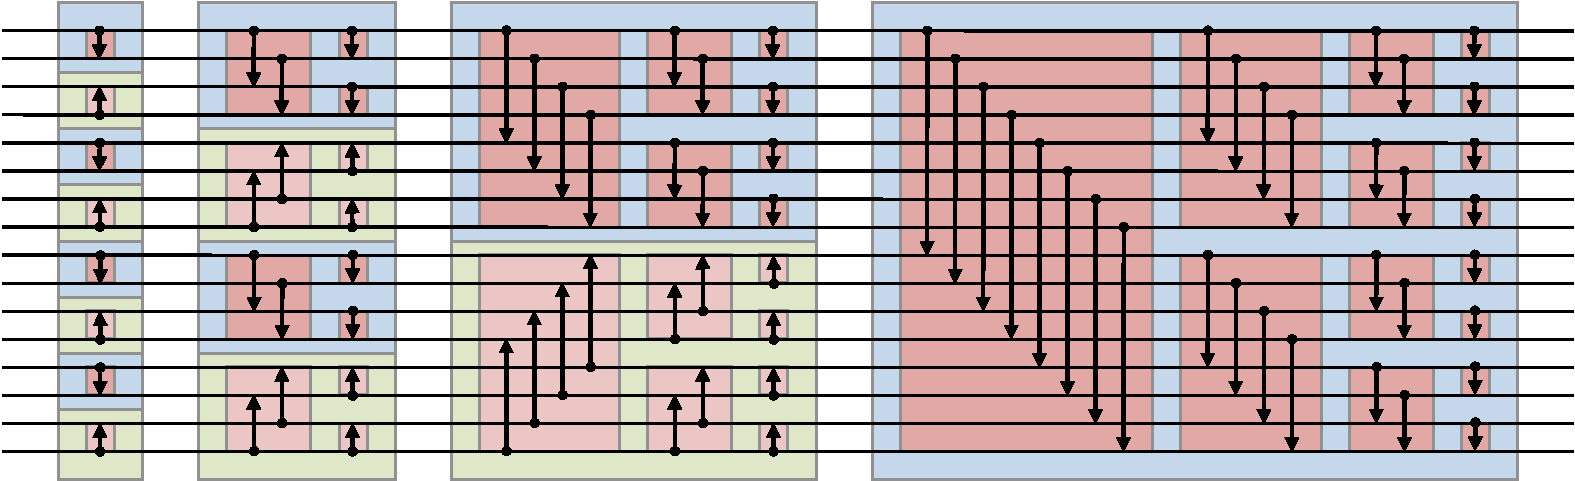
\includegraphics[width=0.8\linewidth]{bitonic_sort}
\caption{Example of a bitonic sorting network for 16 inputs \cite{wiki_bitonic_sort}.}
\label{fig:bitonic_sort}
\end{figure}

approach
kernel code/host code with explanation
improvements
runtime (diagram), $n * n \log^2(n)$, why still faster than CPU?

\lstset{basicstyle=\ttfamily{}\scriptsize{}}
\lstinputlisting[language=C++, caption=Host code for a bitonic sort implementation. The implementation is based on an article about experiences with OpenCL and sorting by Eric Bainville \cite{sort_bealto}., label=lst:sort_bitonic_host, firstline=106, lastline=142]{code/sort/main.cpp}
\lstset{basicstyle=\ttfamily{}}

\lstset{basicstyle=\ttfamily{}\scriptsize{}}
\lstinputlisting[language=CL, caption=OpenCL Kernel code for one iteration of a bitonic sort. The implementation is based on an article about experiences with OpenCL and sorting by Eric Bainville \cite{sort_bealto}. , label=lst:sort_bitonic_kernel,]{../src/sort/gpu/thesis/BitonicSort.cl}
\lstset{basicstyle=\ttfamily{}}

\subsubsection{Bitonic Sort using kernel fusion}



\lstset{basicstyle=\ttfamily{}\scriptsize{}}
\lstinputlisting[language=C++, caption=Host code for a bitonic sort implementation using kernel fusion. The implementation is based on an article about experiences with OpenCL and sorting by Eric Bainville \cite{sort_bealto}., label=lst:sort_bitonic_fusion_host, firstline=144, lastline=209]{code/sort/main.cpp}
\lstset{basicstyle=\ttfamily{}}

\lstset{basicstyle=\ttfamily{}\scriptsize{}}
\lstinputlisting[language=CL, caption={OpenCL code of several kernels performing 1,2,4 or 8 iterations of a bitonic sort. The implementation is based on an article about experiences with OpenCL and sorting by Eric Bainville \cite{sort_bealto}.} , label=lst:sort_bitonic_fusion_kernel,]{../src/sort/gpu/thesis/BitonicSortFusion.cl}
\lstset{basicstyle=\ttfamily{}}

\subsubsection{Radix Sort}
\label{sec:sorting_radix}
integer only
seems easy to parallelize, problems? (order of work item execution)

kernel code/ host code (AMD/NVIDIA)

\lstset{basicstyle=\ttfamily{}\scriptsize{}}
\lstinputlisting[language=C++, caption=Host code for a radix sort implementation. The implementation is based on the radix sort sample shipped with AMD APP SDK \cite{amd_app_sdk}., label=lst:sort_radix_host, firstline=301, lastline=361]{code/sort/main.cpp}
\lstset{basicstyle=\ttfamily{}}

\lstset{basicstyle=\ttfamily{}\scriptsize{}}
\lstinputlisting[language=CL, caption=OpenCL code for the histogram and permute kernels  of a radix sort. Each work item stores it's histogram in registers. The implementation is based on the radix sort sample shipped with AMD APP SDK \cite{amd_app_sdk}. , label=lst:sort_radix_kernel, lastline=41]{../src/sort/gpu/thesis/RadixSort.cl}
\lstset{basicstyle=\ttfamily{}}

\subsubsection{Radix Sort using local memory}


\lstset{basicstyle=\ttfamily{}\scriptsize{}}
\lstinputlisting[language=C++, caption=Changes to the host code of listing \ref{lst:sort_radix_host} for a radix sort implementation using local memory to store each thread's histogram. The implementation is based on the radix sort sample shipped with AMD APP SDK \cite{amd_app_sdk}., label=lst:sort_radix_local_host, firstline=425, lastline=429]{code/sort/main.cpp}
\lstset{basicstyle=\ttfamily{}}

\lstset{basicstyle=\ttfamily{}\scriptsize{}}
\lstinputlisting[language=CL, caption=OpenCL code for the histogram and permute kernels  of a radix sort. Each work item stores it's histogram in local memory. The implementation is based on the radix sort sample shipped with AMD APP SDK \cite{amd_app_sdk}. , label=lst:sort_radix_local_kernel, lastline=46]{../src/sort/gpu/thesis/RadixSortLocal.cl}
\lstset{basicstyle=\ttfamily{}}

\subsection{Existing implementations}
libCL
AMD APP SDK Samples
NVIDIA OpenCL Samples
clpp
